\documentclass{article}
\usepackage{graphicx, float, url, hyperref, afterpage, amsthm, amsmath, listings, pdflscape}

\title{Training Artificial Neural Networks on Unbalanced Data}
\author{Joshua Frankie Rayo\\2011-19612\\CS 280 Programming Assignment 2}
\date{\today}

\begin{document}

\maketitle
\tableofcontents

\section{Introduction}
	This work deals with using artificial neural networks as an intelligent system for classifying objects that is trained under highly unbalanced dataset. An approach to train the network is to generate data from what is already given. To upsample the dataset, SMOTE (Synthetic Minority Over-sampling Technique) algorithm has been used. Training parameters are tweaked to make good results in training and validation and to check the respective errors if they are as low as possible. The parameters include number of nodes in each layer, learning rate, and error tolerance criterion. The program is implemented using Python and NumPy package to enable code vectorization and make computations faster.

\section{Methodology}
The neural network is made using Python which is a high level, general-purpose programming language relatively easy to learn and has very good features in list manipulation and vectorized computations. Also, the syntax for matrix computations of NumPy package is quite similar to MATLAB\cite{bib:mat}.

\subsection{Dealing with Unbalanced Data}
In the given dataset there are classes that have more instances than others. What does it mean to train an unbalanced data? Training the neural network with this kind of data might lead to overfitting and tend to assign objects in the dominant class most of the time\cite{bib:imb}. This might lead to high accuracy but having a model with high accuracy is not really effective in prediction, which is known as the \textit{accuracy paradox}\cite{bib:acp}.

There are several approaches in dealing with unbalanced data\cite{bib:unb} (but is not limited to the following):
\begin{itemize}
	\item Gather more data as much as possible
	\item Resample the dataset, meaning to generate new data
	\item Downsample the dataset, meaning to remove some instances
	\item Upsample the dataset, meaning to generate synthetic samples from the existing data
	\item Use a cost-sensitive classifier to minimize misclassification of the different classes
\end{itemize}

One of these approaches can be adapted depending on the given dataset and other restrictions. Gathering more data or resampling is impossible because its source is of unknown nature. There is nothing that can be inferred physically given only a sequence of numbers. Moreover, using a cost-sensitive classifier is not favorable since we do not know what penalty costs will be assigned for each misclassification. Downsampling the dataset is risky since there might be very important instances that might be removed. Therefore upsampling the dataset is the most feasible of the approaches given above. The SMOTE (Synthetic Minority Over-sampling Technique) algorithm is an upsampling approach which make data distribution more balanced by generating more instances from the minority classes as outlined by the algorithm below\cite{bib:smote}.

\begin{enumerate}
	\item Take the difference between the feature vector under consideration and its nearest neightbor that belongs on the same class.
	\item Multiply this difference by a random number between 0 and 1 and add it to the feature vector under the same class.
\end{enumerate}

Mathematically, the synthetic instance is represented as $x_{new} = x_{1} + \text{rand}(0,1) * x_{2}$ where $x_{1}, x_{2}$ are neighboring features that belong to the same class. There are many ways to define a 'neighbor', perhaps through a distance function which can be Euclidean or $L_1$-norm distance. This causes the selection of a random point along the line segment between two specific features. In effect, it forces the decision region of the minority class to become more general\cite{bib:smote}.

In this particular work, synthetic instances are generated from the minority classes to make all class instances equal in population. The distance function used in determining nearby vectors is the $L_1$-norm condition defined as $\sum_{i=0}^{n} \left\| x(i) - y(i) \right\| < 0.001$.

The table below show statistics regarding the dataset given and the number of generated instances per class:

\begin{table}[H]
	\centering
	\begin{tabular}{c | c | c | c}
		label & count & generated & total\\
		\hline
		1 & 1625 & 0 & 1625\\
		2 & 233 & 1392 & 1625\\
		3 & 30 & 1595 & 1625\\
		4 & 483 & 1142 & 1625\\
		5 & 287 & 1338 & 1625\\
		6 & 310 & 1315 & 1625\\
		7 & 52 & 1573 & 1625\\
		8 & 466 & 1159 & 1625\\
		total & 3486 & 9514 & \textbf{13000}\\
	\end{tabular}
\end{table}

\subsection{Dataset Partitioning}

After using SMOTE algorithm, the total number of instances is now 13,000 with each of the classes equally represented. The new dataset is divided into two partitions A and B. Partition A consists of 6,500 instances that includes original and synthetic data while partition B also have 6,500 instances that are all synthetic. The former is used for training and the latter is used for validating the network. In this manner the original data is still be used for training the network and original information are taken into account.

\subsection{Network Learning}

There are several parameters to be considered in training the network:
\begin{itemize}
	\item Number of input neurons
	\item Number of hidden layers
	\item Number of neurons per layer
	\item Number of output neurons
	\item Learning rate $\eta$
	\item Error tolerance $\hat{J}$
\end{itemize}

The number of input neurons is set to 354, which is the number of features in an instance, while the number of output neurons is 3 which can represent 8 classes in binary form. The number of hidden layers are fixed into two. These values are specific to this particular problem. The learning rate is set to 1.0 which is the rate of gradient descent. Larger learning rate is being more aggressive in finding a minimum.

In setting the number of nodes in the hidden layers, it is suggested from \cite{bib:pat} that the number of synaptic weights should be large enough to learn similarities of the instances that belong to same class and small enough to learn the differences of these similar instances. Moreover, the neurons of the first layer form the hyperplanes that separates the points, those from the second layer form the regions and the output layer form the classes\cite{bib:pat}. Since there are only 8 classes, having 8 neurons in the first (8 separating hyperplanes) and second layers (8 sets of regions) is a good choice. However, both has been increased to 16 hoping that the network might capture the bigger picture as much as possible. In simulating the network, there is no significant gain in accuracy using only 8 nodes or 16 nodes at both layers.

The error in each instance $i$ is defined as the sum of squared errors in output $\epsilon(i) = \frac{1}{2}\left\| \mathbf{y}-\mathbf{\hat{y}} \right\|^2$, while the error in an epoch is the sum of errors from $m$ instances $J = \sum_{i=0}^{m}\epsilon(i)$. The sample code needs to be modified since it only checks for the last error in an epoch and not the sum.

In training the network, random values are assigned for weights and biases generated from the uniform distribution centered at -0.5. For each epoch, instances are drawn at random without replacement to make sure the network will not deduce any pattern that can produce bias during prediction. The labels (1-8) are of course converted to its binary representation (000-111) to be accepted by the network. For producing output, each neuron will be assigned 1 if its value is greater than 0.5 and 0 otherwise. Note that this is binary again and shall be converted back to its decimal representation for the final class labeling.

\section{Discussion of Results}

The network is ran using a laptop with Kali Linux OS, 8Gb RAM and Intel Core i3 @ 2.10GHz x 4 processors.For each epoch, training error for partition A and validation error for partition B is computed. The latter is computed as the percentage of misclassification in the validation set. In training the network, it is observed that the errors are large since each instance has 354 features and the cost function is quadratic. The figure below shows learning with $\hat{J}=300$ and $\eta=1.5$.

\begin{landscape}
	\begin{figure}[H]
		\centering
		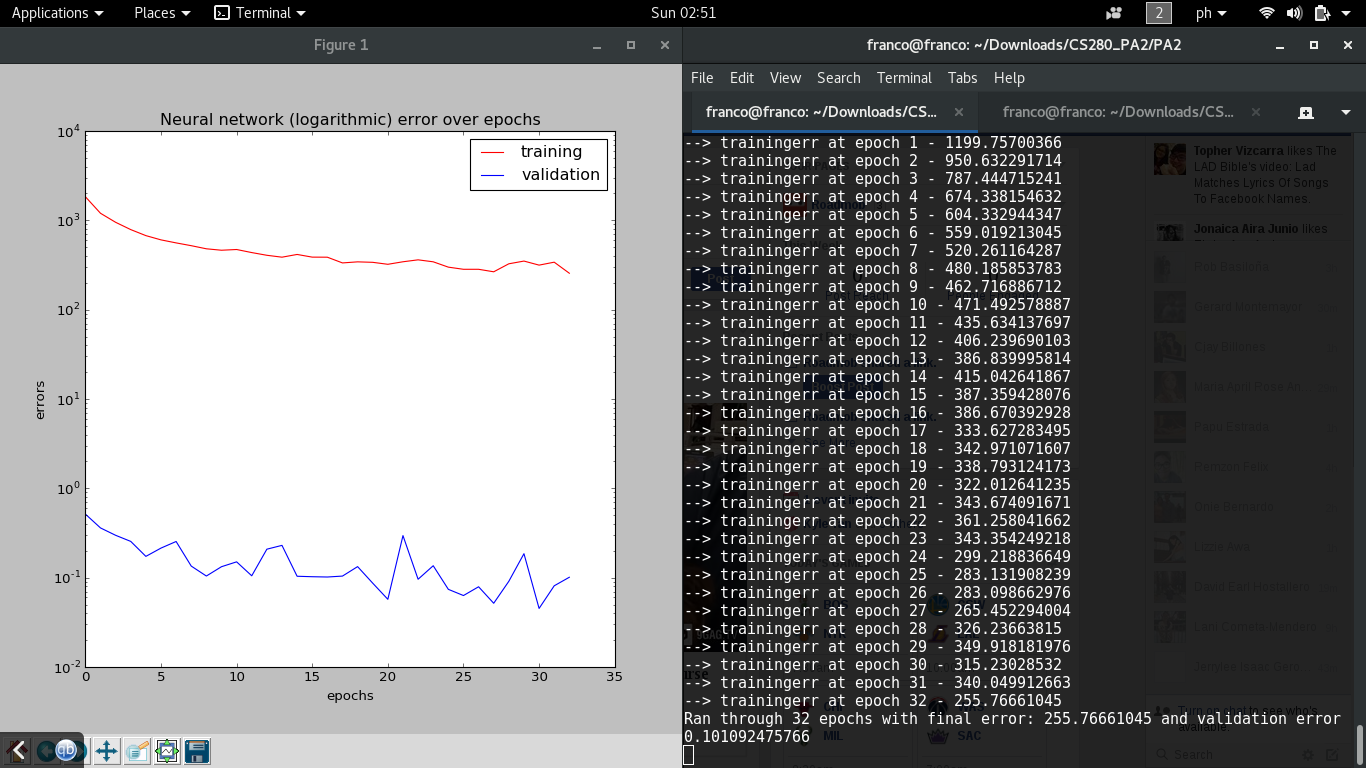
\includegraphics[width=1.6\textwidth]{1,5,300}
	\end{figure}
	At first, training error quickly decrease and began oscillating at $J\approx 200-300$ in searching for the minimum. In this situation the local minimum is within that region and the gradient descent algorithm searches for a better estimate relative to error tolerance. The next figure below shows a simulation where $\hat{J}=250$ and $\eta=1.5$


	\begin{figure}[H]
		\centering
		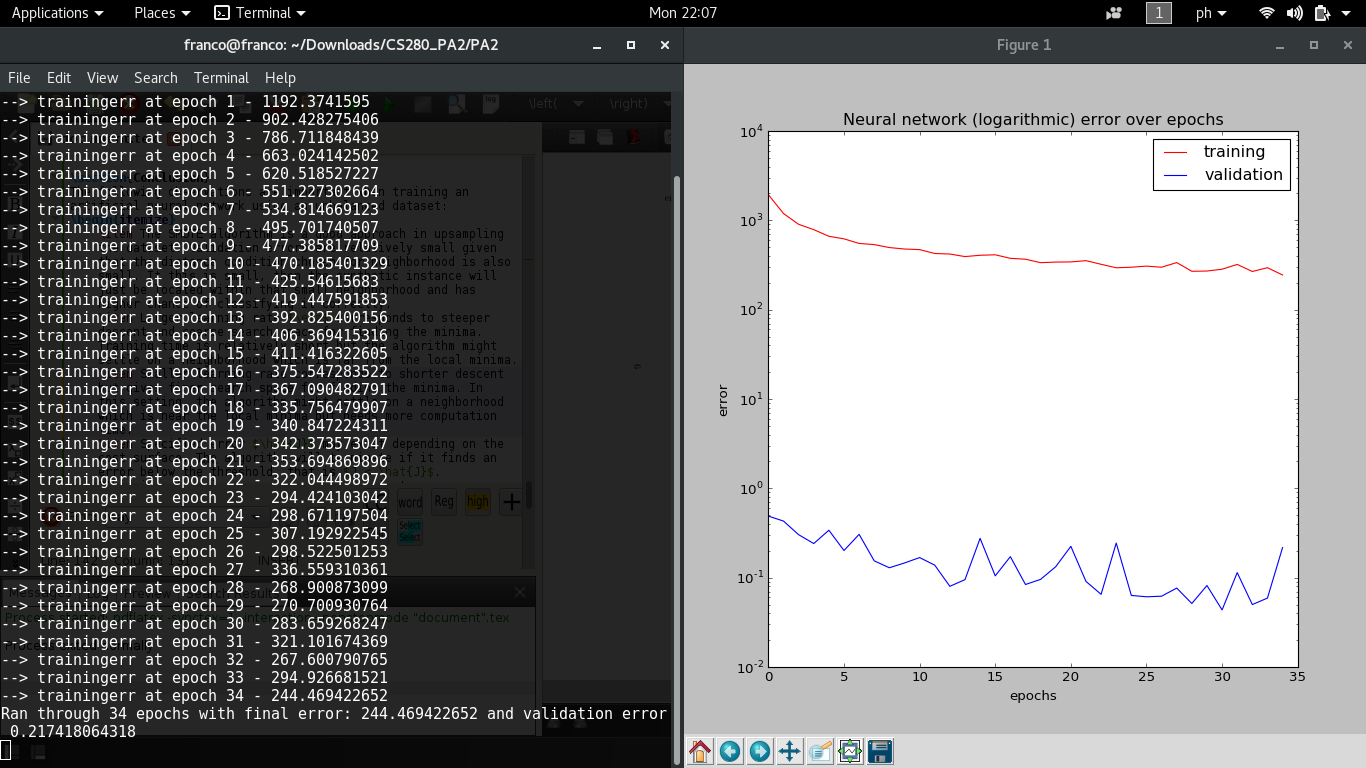
\includegraphics[width=1.5\textwidth]{1,5,250}
	\end{figure}

	Training time increases if the learning rate is small and the algorithm is not much aggressive. If error tolerance (proposed minimum) is set to $\hat{J}=100$ or sufficiently small number, the algorithm may not terminate because this minimum might not exist depending on the cost surface. Small learning rate means finer search space in finding the minimum thus more time is required. The figure below shows a simulation where $\hat{J}=150$, $\eta=0.5$:
	\begin{figure}[H]
		\centering
		\includegraphics[width=1.5\textwidth]{point5,150}
	\end{figure}

	In this realization where $\hat{J}=100$ and $\eta=0.5$, learning takes 74 epochs with training error of 94.6953 and validation error of 0.0491.
	\begin{figure}[H]
		\centering
		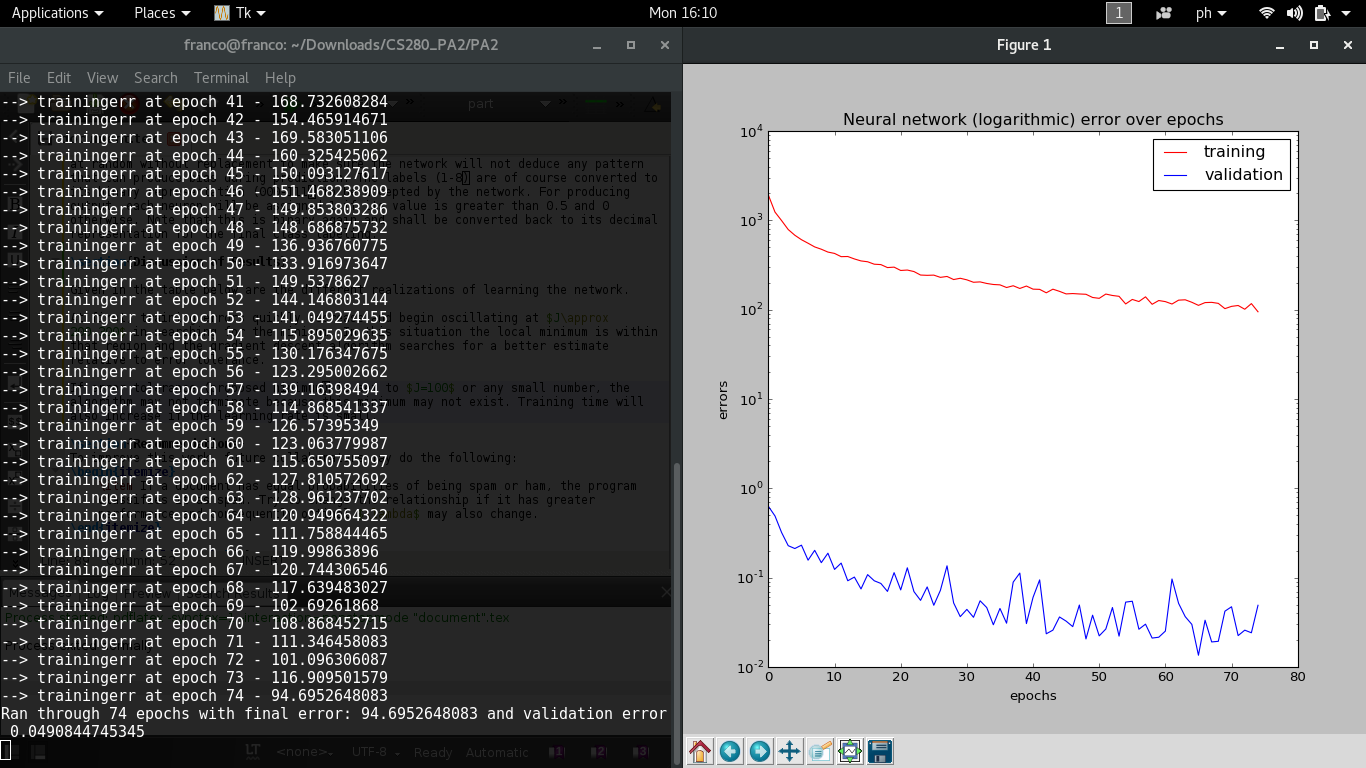
\includegraphics[width=1.6\textwidth]{point5,100}
	\end{figure}

	This might ring bells: small validation error means great accuracy. But as you can see the graph, the validation error decreases at first then reaches minimum but tends to grow again with rapid oscillations. This is a sign of overfitting the dataset. Another instance that leads to this situation is having $\hat{J} = 100$ and $\eta=0.05$ as given in the figure below.
	\begin{figure}[H]
		\centering
		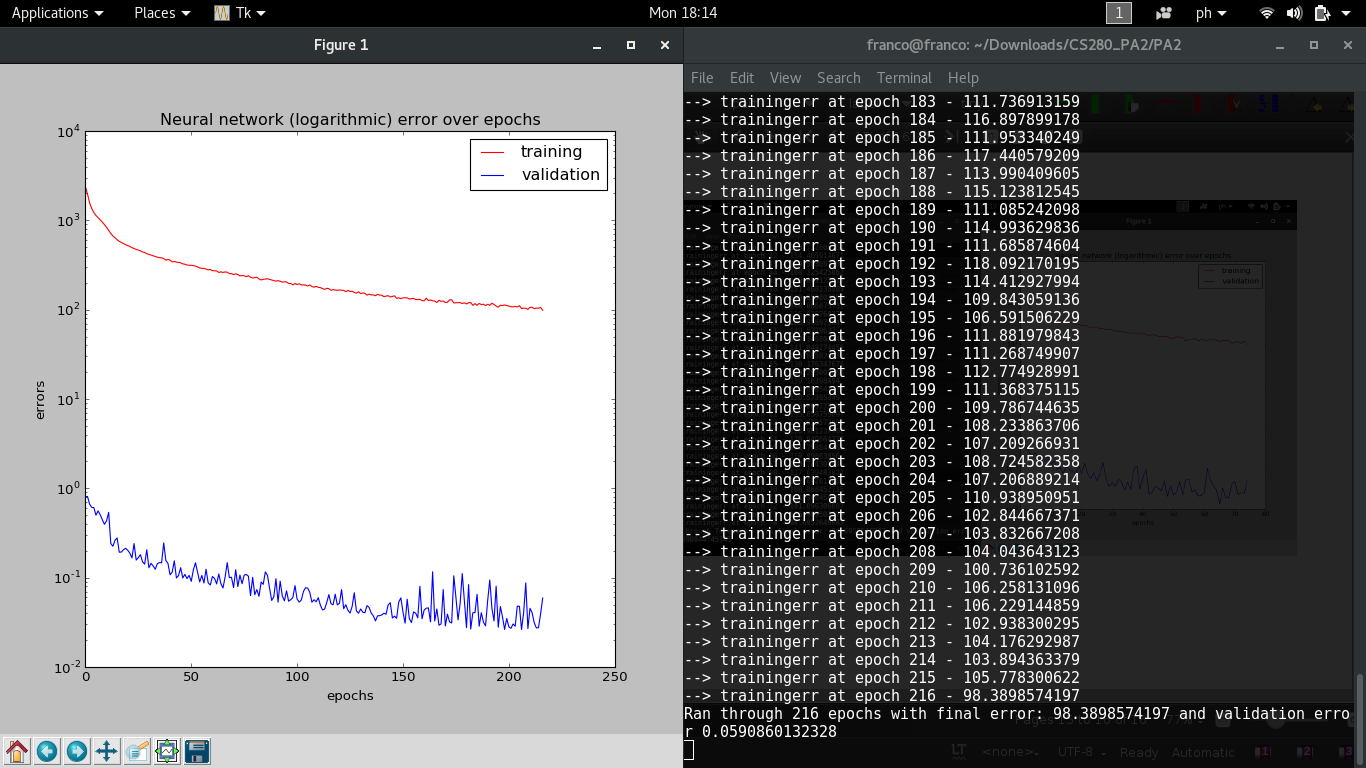
\includegraphics[width=1.5\textwidth]{0,5,100}
	\end{figure}
	
	In this situation where overfitting is evident, one must settle on higher error tolerance so that prediction will be better. Lastly, the figure below shows a simulation with recommended parameters $\hat{J}=200$ and $\eta=0.5$. 
	This shows an error of 197.6346 and validation error of 0.0413 in 32 epochs.
	\begin{figure}[H]
		\centering
		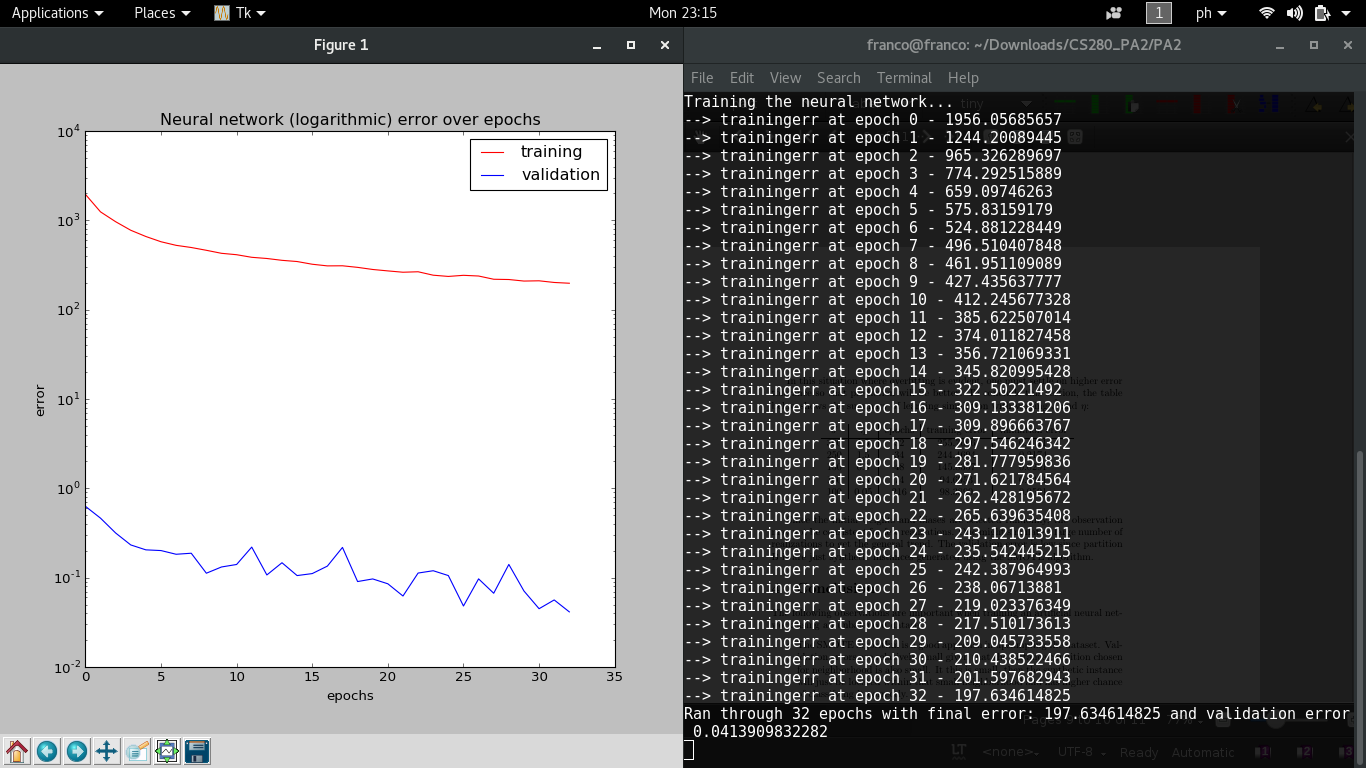
\includegraphics[width=1.5\textwidth]{0,5,200}
	\end{figure}
\end{landscape}


To conclude this section, the table below shows the summary of learning simulation with varying $\hat{J}$ and $\eta$:

\begin{table}[H]
	\centering
	\begin{tabular}{c | c | c | c | c}
		$\hat{J}$ & $\eta$ & epochs & training error & validation error\\
		\hline
		300 & 1.5 & 32 & 255.7666 & 0.1011\\
		250 & 1.5 & 34 & 244.4694 & 0.2174\\
		200 & 0.5 & 32 & 197.6346 & 0.0413\\
		150 & 0.5 & 48 & 145.8357 & 0.0291\\
		100 & 0.5 & 74 & 94.6953 & 0.0491\\
		100 & 0.05 & 216 & 98.3899 & 0.0591\\
	\end{tabular}
\end{table}

Since the initial weights and biases are selected randomly, the observations may not be consistent for few realizations. One might simulate a large number of realizations to get the general trend. The validation error is low since partition B is are just synthetic instances generated using the SMOTE algorithm. At this point, unbalanced data has been addressed and finally the neural network is now ready for prediction.

\section{Conclusion}
The following observations are important when training an artificial neural network using an unbalanced dataset:
\begin{itemize}
	\item The SMOTE algorithm is a good approach in upsampling the dataset. Validation errors are relatively small given that the distance condition chosen for neighborhood is also small. The synthetic instance will just be located within that small neighborhood and has higher chance of classifying it correctly.
	\item Larger learning rate $\eta$ corresponds to steeper descent and coarse search space for finding the minima. Training time is relatively short but the algorithm might settle on a neighborhood which is far from the local minima.
	\item Smaller learning rate corresponds to shorter descent but gives finer search space for finding the minima. In this situation, the algorithm might settle on a neighborhood which is near the local minima. More computation time is needed to get better results.
	\item Specified error $\hat{J}$ may exist depending on the cost surface. The algorithm will terminate if it finds an error below the threshold, that is $J < \hat{J}$. Otherwise, learning process may not terminate.
	\item The number of nodes in the hidden layer determines the separation of points and classes of the unions of regions in the corresponding hyperspace. Increasing the network size may not necessarily improve its prediction performance. Moreover, having large network size needs more memory and computational time.
\end{itemize}

\begin{thebibliography}{9}
	\bibitem{bib:imb}
	Jason Brownlee. \emph{8 Tactics to Combat Imbalanced Classes in Your
		Machine Learning Dataset}. \url{http://machinelearningmastery.com/tactics-to-combat-imbalanced-classes-in-your-machine-learning-dataset/}
	
	\bibitem{bib:acp}
	TryoLabs. \emph{Why accuracy alone is a bad measure for classification tasks, and what we can do about it}. \url{https://tryolabs.com/blog/2013/03/25/why-accuracy-alone-bad-measure-classification-tasks-and-what-we-can-do-about-it/}
	
	\bibitem{bib:smote}
	N. V. Chawla, et. al. \emph{SMOTE: Synthetic Minority Over-sampling Technique}. \url{http://www.jair.org/papers/paper953.html}
	
	\bibitem{bib:unb}
	\emph{Which classifi ers work well with unbalanced data?} \url{http://stats.stackexchange.com/questions/109177/which-classifiers-work-well-with-unbalanced-data?rq=1}
	
	\bibitem{bib:pat}
	Theodoridis, Koutroumbas. \emph{Pattern Recognition}, 4th ed. 2008
	
	\bibitem{bib:mat}
	The Scipy community. \emph{NumPy for MATLAB users}. \url{http://docs.scipy.org/doc/numpy-dev/user/numpy-for-matlab-users.html}
\end{thebibliography}

\end{document}
